\documentclass{article}
\usepackage{amsmath}
\usepackage{amssymb}
\usepackage{zed-csp} % Paquete Z
\usepackage[T1]{fontenc}
\usepackage{indentfirst}
\usepackage{mathtools}
\usepackage{xparse} 
\usepackage{fancyhdr}
\usepackage[spanish]{babel}
\usepackage[font=small,labelfont=bf]{caption}
\usepackage[a4paper,hmargin=1in, vmargin=1.4in,footskip=0.25in]{geometry}

\usepackage{z-eves}

\usepackage{framed}
\newcommand{\desig}[2]{\item #1 $\approx #2$}
\newenvironment{designations}
  {\begin{leftbar}
    \begin{list}{}{\setlength{\labelsep}{0cm}
                   \setlength{\labelwidth}{0cm}
                   \setlength{\listparindent}{0cm}
                   \setlength{\rightmargin}{\leftmargin}}}
  {\end{list}\end{leftbar}}


\setlength{\parskip}{8pt}

% defining command for the curly arrow
\newcommand{\curly}{\mathrel{\leadsto}}

\DeclarePairedDelimiterX{\Iintv}[1]{\llbracket}{\rrbracket}{\iintvargs{#1}}
\NewDocumentCommand{\iintvargs}{>{\SplitArgument{1}{,}}m}
{\iintvargsaux#1}
\NewDocumentCommand{\iintvargsaux}{mm} {#1\mkern1.5mu,\mkern1.5mu#2}

\makeatletter
\newcommand*{\currentname}{\@currentlabelname}
\makeatother

\addtolength{\textwidth}{0.2cm}
\setlength{\parskip}{8pt}
\setlength{\parindent}{0.5cm}
\linespread{1.5}

\pagestyle{fancy}
\fancyhf{}
\rhead{TP - Sullivan}
\lhead{Ingeniería de Software}
\rfoot{\vspace{1cm} \thepage}

\renewcommand*\contentsname{\LARGE Índice}

\begin{document}

\begin{titlepage}
    \begin{center}
        \vfill
        \vfill
            \vspace{0.7cm}
            \noindent\textbf{\Huge Trabajo Práctico \\ Verificación de Software}\par
            \vspace{.5cm}
        \vfill
        \noindent \textbf{\huge Alumna:}\par
        \vspace{.5cm}
        \noindent \textbf{\Large Sullivan, Katherine}\par
 
        \vfill
        \large Universidad Nacional de Rosario \par
        \noindent\large 2024
    \end{center}
\end{titlepage}
\ \par

\vspace{-2cm}

\section*{El problema: Sistema de Gestión de Cursos de Universidad}

Se requiere la construcción de un sistema de gestión de cursos de universidad. El mismo debe ser capaz de asignar profesores a un curso, anotar alumnos a cursos para los cuales ya se encuentren asignados profesores y mostrar información de cursos existentes en la universidad.

\section*{Designaciones}

\begin{designations}
\desig{$s$ es un estudiante}{s \in STUDENT}
\desig{$p$ es un profesor}{p \in PROFESSOR}
\desig{$c$ es un identificador de curso}{c \in COURSE}
\desig{Conjunto de estudiantes anotados en el curso $c$}{enrolledStudents(c)}
\desig{Conjunto de profesores asignados al curso $c$}{assignedProfessors(c)}
\end{designations}

\section*{Especificación Z}

\begin{zed}
[STUDENT, PROFESSOR, COURSE]
\end{zed}

\begin{schema}{CourseManagementSystem}
    enrolledStudents: COURSE \pfun \power STUDENT \\
    assignedProfessors: COURSE \pfun \power PROFESSOR
\end{schema}

\begin{schema}{CourseManagmentInit}
CourseManagementSystem
\where
    enrolledStudents = \emptyset \\
    assignedProfessors = \emptyset
\end{schema}

Invariante: un estudiante no se puede anotar a un curso que no tenga profesores asignados todavía.

\begin{schema}{CourseManagmentInv}
CourseManagementSystem
\where
    \dom(enrolledStudents) \subseteq \dom(assignedProfessors)
\end{schema}

Operación que permite anotar un alumno a un curso: \textit{EnrollStudent}.

\begin{schema}{EnrollStudentOldCourseOk}
    \Delta CourseManagementSystem \\
    student?: STUDENT \\
    course?: COURSE
    \where
    course? \in \dom(assignedProfessors) \\
    course? \in \dom(enrolledStudents) \\
    student? \notin enrolledStudents(course?) \\
    enrolledStudents' = enrolledStudents \oplus \{course? \mapsto (enrolledStudents(course?) \cup \{student?\})\} \\
    assignedProfessors' = assignedProfessors
\end{schema}

\begin{schema}{StudentAlreadyInCourse}
\Xi CourseManagementSystem \\
student?: STUDENT \\
course?: COURSE 
\where
    course? \in \dom(assignedProfessors) \\
    course? \in \dom(enrolledStudents) \\
    student? \in enrolledStudents(course?)
\end{schema}

\begin{schema}{EnrollStudentNewCourseOk}
    \Delta CourseManagementSystem \\
    student?: STUDENT \\
    course?: COURSE
    \where
    course? \in \dom(assignedProfessors) \\
    course? \nin \dom(enrolledStudents) \\
    enrolledStudents' = enrolledStudents \cup \{course? \mapsto \{student?\}\} \\
    assignedProfessors' = assignedProfessors
\end{schema}

\begin{schema}{CourseNotReady}
\Xi CourseManagementSystem \\
course?: COURSE
\where
    course? \nin \dom(assignedProfessors)
\end{schema}

\begin{zed}
    EnrollStudent == EnrollStudentOldCourseOk  \lor EnrollStudentNewCourseOk \lor CourseNotReady \\ \hspace{2.5cm} \lor StudentAlreadyInCourse
\end{zed}

Operación que permite asignar profesores a un curso: \textit{AssignProfessor}.

\begin{schema}{AssignProfessorsOk}
    \Delta CourseManagementSystem \\
    professors?: \power PROFESSOR \\
    course?: COURSE
    \where
    course? \notin \dom(assignedProfessor) \\
    assignedProfessors' = assignedProfessors \cup \{course? \mapsto professors?\} \\
    enrolledStudents' = enrolledStudents
\end{schema}

\begin{schema}{CourseAlreadyAssigned}
    \Xi CourseManagementSystem \\
    professors?: \power PROFESSOR \\
    course?: COURSE
    \where
    course? \in \dom(assignedProfessors)
\end{schema}

\begin{zed}
    AssignProfessors == AssignProfessorsOk \lor CourseAlreadyAssigned
\end{zed}

Operación que permite mostrar información de un curso: \textit{ShowCourseInfo}.

\begin{schema}{ShowCourseInfoWithStudentsOk}
    \Xi CourseManagementSystem \\
    course?: COURSE \\
    enrolledStudents!: \power STUDENT \\
    assignedProfessors!: \power PROFESSOR
    \where
    course? \in \dom(assignedProfessors) \\
    course? \in \dom(enrolledStudents) \\
    enrolledStudents! = enrolledStudents(course?) \\
    assignedProfessors! = assignedProfessors(course?)
\end{schema}

\begin{schema}{ShowCourseInfoWithoutStudentsOk}
    \Xi CourseManagementSystem \\
    course?: COURSE \\
    enrolledStudents!: \power STUDENT \\
    assignedProfessors!: \power PROFESSOR
    \where
    course? \in \dom(assignedProfessors) \\
    course? \nin \dom(enrolledStudents) \\
    enrolledStudents! = \emptyset \\
    assignedProfessors! = assignedProfessors(course?)
\end{schema}

\begin{schema}{NoInfoToShow}
    \Xi CourseManagementSystem \\
    course?: COURSE \\
    enrolledStudents!: \power STUDENT \\
    assignedProfessor!: \power PROFESSOR
    \where
    course? \nin \dom(assignedProfessors) \\
    enrolledStudents! = \emptyset \\
    assignedProfessor! = \emptyset
\end{schema}

\begin{zed}
    ShowCourseInfo == ShowCourseInfoWithStudentsOk \lor ShowCourseInfoWithoutStudentsOk \\ 
    \hspace{2.90cm} \lor NoInfoToShow
\end{zed}

\subsection*{Especificación Z normalizada}

Teniendo en cuenta lo visto en Ingeniería del Software I, cambiarán las definiciones de las variables de estado y los invariantes, puesto que que en Z las funciones parciales no son un tipo.

\begin{schema}{CourseManagementSystem}
    enrolledStudents: COURSE \rel \power STUDENT \\
    assignedProfessors: COURSE \rel \power PROFESSOR
\end{schema}

\begin{schema}{CourseManagmentInv}
CourseManagementSystem
\where
    \dom(enrolledStudents) \subseteq \dom(assignedProfessors) \\
    enrolledStudents \in COURSE \pfun \power STUDENT \\
    assignedProfessor \in COURSE \pfun PROFESSOR
\end{schema}

\section*{Traducción a \{log\}}

La traducción a \{log\} (aceptada por el typechecker) se encuentra en el archivo \verb|courseMgmt.pl|.

\section*{Ejecución de simulaciones en \{log\}}
Planteamos dos simulaciones: una directa y una inversa. Las presentamos a continuación pero también se encuentran disponibles en el archivo \verb|simulaciones.pl|.

\subsection*{Simulación 1}

Definimos la siguiente simulación directa:

\begin{verbatim}
    dec([P0, P1, P2, P3], ap) & 
    dec([S0, S1, S2, S3, S4, S5], es) & 
    dec([StudentsPedag, StudentsDer, StudentsPsico], ss) & 
    dec([ProfessorsPedag, ProfessorsDer, ProfessorsPsico], pp) & 
    courseMgmtInit(S0, P0) & 
    assignProfessors(P0, {professor:pauloFreire}, course:pedagogiaCritica, P1) & 
    assignProfessors(P1, {professor:savitribaiPhule, professor:simonedeBeauvoir},
                    course:derechosDeLaMujer, P2) & 
    assignProfessors(P2, {professor:jeanPiaget, professor:levVygotsky}, 
                    course:derechosDeLaMujer, P3) & 
    enrollStudent(S0, P3, student:leo, course:epistemologia, S1) & 
    enrollStudent(S1, P3, student:maya, course:derechosDeLaMujer, S2) & 
    enrollStudent(S2, P3, student:maya, course:pedagogiaCritica, S3) & 
    enrollStudent(S3, P3, student:leo, course:pedagogiaCritica, S4) & 
    enrollStudent(S4, P3, student: leo, course:psicopedagogia, S5) & 
    showCourseInfo(S5, P3, course:pedagogiaCritica, StudentsPedag, ProfessorsPedag) & 
    showCourseInfo(S5, P3, course:derechosDeLaMujer, StudentsDer, ProfessorsDer) & 
    showCourseInfo(S5, P3, course:psicopedagogia, StudentsPsico, ProfessorsPsico).
\end{verbatim}

y obtenemos el resultado esperado (único):

\begin{verbatim}
    P0 = {},  
    P1 = {[course:pedagogiaCritica,{professor:pauloFreire}]},  
    P2 = {[course:pedagogiaCritica,{professor:pauloFreire}],
        [course:derechosDeLaMujer,{professor:savitribaiPhule,professor:simonedeBeauvoir}]},  
    P3 = {[course:pedagogiaCritica,{professor:pauloFreire}],
        [course:derechosDeLaMujer,{professor:savitribaiPhule,professor:simonedeBeauvoir}]},  
    S0 = {},  
    S1 = {},  
    S2 = {[course:derechosDeLaMujer,{student:maya}]},  
    S3 = {[course:pedagogiaCritica,{student:maya}],[course:derechosDeLaMujer,{student:maya}]},  
    S4 = {[course:derechosDeLaMujer,{student:maya}],
        [course:pedagogiaCritica,{student:leo,student:maya}]},  
    S5 = {[course:derechosDeLaMujer,{student:maya}],
        [course:pedagogiaCritica,{student:leo,student:maya}]},  
    StudentsPedag = {student:leo,student:maya},  
    StudentsDer = {student:maya},  
    StudentsPsico = {},  
    ProfessorsPedag = {professor:pauloFreire},  
    ProfessorsDer = {professor:savitribaiPhule,professor:simonedeBeauvoir},  
    ProfessorsPsico = {}

\end{verbatim}

\subsection*{Simulación 2}

Generamos la siguiente simulación inversa:

\begin{verbatim}
    dec([P0, P1, P2], ap) & 
    dec([S0, S1, S2], es) & 
    dec([Course1, Course2], course) & 
    dec([Profs1, Profs2], pp) & 
    dec([Student1, Student2], student) & 
    assignProfessors(P0, Profs1, Course1, P1) & 
    assignProfessors(P1, Profs2, Course2, P2) & 
    enrollStudent(S0, P2, Student1, Course1, S1) & 
    enrollStudent(S1, P2, Student2, Course2, S2) & 
    P2 = {[course:fonoaudiologia, {professor:mariaMontessori}], 
        [course:literatura, {professor:juanaManso}]} & 
    S2 = {[course:fonoaudiologia, {student:ailen}], 
        [course:literatura, {student:camila}]}.
\end{verbatim}

y la primer solución obtenida es:

\begin{verbatim}
    P0 = {},  
    P1 = {[course:fonoaudiologia,{professor:mariaMontessori}]},  
    P2 = {[course:fonoaudiologia,{professor:mariaMontessori}],
        [course:literatura,{professor:juanaManso}]},  
    S0 = {[course:fonoaudiologia,{}],[course:literatura,{}]/_N2},  
    S1 = {[course:fonoaudiologia,{student:ailen}],[course:literatura,{}]/_N1},  
    S2 = {[course:fonoaudiologia,{student:ailen}],
        [course:literatura,{student:camila}]},  
    Course1 = course:fonoaudiologia,  
    Course2 = course:literatura,  
    Profs1 = {professor:mariaMontessori},  
    Profs2 = {professor:juanaManso},  
    Student1 = student:ailen,  
    Student2 = student:camila
    Constraint: dom(_N2,_N6), set(_N6), 
    [course:fonoaudiologia,{}]nin _N5, set(_N5), 
    un(_N5,_N1,_N2), set(_N2), dom(_N5,_N4), rel(_N5), set(_N4), 
    subset(_N4,{course:fonoaudiologia}), course:fonoaudiologia nin _N3, 
    [course:fonoaudiologia,{}]nin _N2,
    comp({[course:fonoaudiologia,course:fonoaudiologia]},_N2,{}), rel(_N2), 
    [course:fonoaudiologia,{student:ailen}]nin _N1, dom(_N1,_N3), set(_N3), 
    subset(_N3,{course:literatura}), set(_N1), [course:literatura,{}]nin _N1, 
    comp({[course:literatura,course:literatura]},_N1,{}), rel(_N1)
\end{verbatim}

\section*{Generado de las condiciones de verificación}

En la versión final del archivo el comando \verb|check_vcs_courseMgmt| realiza todas las descargas de prueba automáticamente y no fue necesario agregar ninguna hipótesis.

\subsection*{Sobre la interacción con el VCG}

En una versión anterior, para las suboperaciones de enrollStudent y assignProfessors que no cambiaban el estado, no tuve en cuenta el poner como parámetro la variable de estado actualizada (EStudents\_ y AProfessors\_, respectivamente) y agregar la sentencia \verb|Var_ = Var| porque pensé que podía obviarlo.

En esta primera versión luego de ver que fallaban los invariantes relacionados con estas operaciones, usé el comando \verb|findh|, que, con razón, me devolvió la lista vacía para las hipótesis faltantes en cada caso. Una vez añadido lo explicado en el párrafo anterior las descargas de prueba fueron automáticas y no fue necesario volver a usar el comando.

\section*{Demostración de lema de invariancia con Z/EVES}

Decidí probar el siguiente teorema:

\begin{theorem}{EnrollCourseMgmtInv}
CourseManagementInv \land EnrollStudent \implies CourseManagementInv'
\end{theorem}

realizando la siguiente prueba:

\begin{zproof}[EnrollCourseMgmtInv]
    split EnrollStudentNewCourseOk;
    cases;
    reduce;
    equality substitute enrolledStudents';
    reduce;
    next;
    split EnrollStudentOldCourseOk;
    cases;
    reduce;
    equality substitute enrolledStudents';
    reduce;
    next;
    split CourseNotReady;
    cases;
    reduce;
    next;
    reduce;
    next;
\end{zproof}

que simplemente consiste en separar la prueba por casos, en cada uno de ellos aplicar reducciones, y en los dos casos donde se modifica la varible de estado enrolledStudents hacer el reemplazo de la versión modificada de la variable por su definición y volver a reducir.

\section*{Generación de casos de prueba con \textsc{Fastest}}

\subsection*{Comandos corridos para obtener los casos de prueba}

\begin{verbatim}
    loadspec fastest.tex
    selop EnrollStudent
    genalltt
    addtactic EnrollStudent_DNF_1 SP \oplus enrolledStudents \oplus 
        \{course? \mapsto (enrolledStudents(course?) \cup \{student?\})\}
    addtactic EnrollStudent_DNF_2 SP \cup 
        enrolledStudents \cup \{course? \mapsto \{student?\}\}
    addtactic EnrollStudent_DNF_3 SP \notin course? \notin \dom assignedProfessors
    addtactic EnrollStudent_DNF_4 SP \in student? \in enrolledStudents~course?
    genalltt
    genalltca    
\end{verbatim}

Lo que hicimos con estos comandos fue primero cargar la especificación desde el archivo, setear la operación para la cual queremos generar los casos de pruebas y, luego, aplicar la primera táctica que se aplica por defecto en  \textsc{Fastest} al correr \verb|genalltt|: la táctica que lleva nuestra operación a su forma normal disyuntiva (DNF). Esto hace que el VIS quede particionado según las precondiciones de las 4 suboperaciones que definimos (EnrollStudentOldCourseOk, EnrollStudentNewCourseOk, CourseNotReady y StudentAlreadyInCourse). Una vez obtenido este árbol, agregamos a la lista de tácticas a ser aplicadas particiones estándar para distintos operadores para las distintas hojas del árbol que habíamos obtenido y volvemos a generar el árbol para el cual si ejecutamos el comando \verb|showtt| obtenemos el siguiente resultado:

\begin{center}
    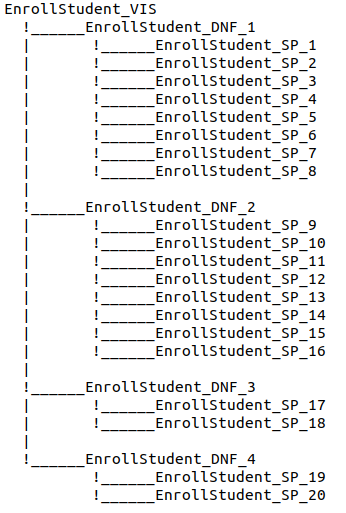
\includegraphics[scale=0.5]{arboltt.png}
    \captionof{figure}{Árbol de prueba luego de ejecutar las tácticas}
\end{center}

Una vez obtenido este árbol, ya sí procedemos con la generación de los casos de prueba, obteniendo el siguiente árbol si corremos \verb|showtt| luego de \verb|genalltca|:

\begin{center}
    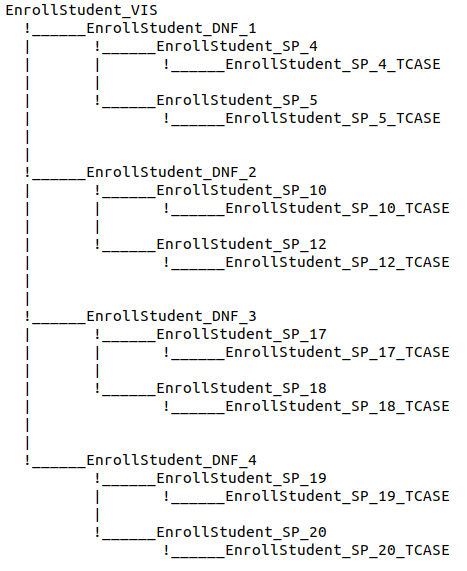
\includegraphics[scale=0.5]{arboltca.png}
    \captionof{figure}{Árbol de prueba luego de obtener los casos de prueba abstractos}
\end{center}


\subsection*{Pero, ¿y las particiones que faltan?}

Rápidamente nos podemos dar cuenta de que los subárboles correspondientes a \verb|EnrollStudent_DNF_1| y \verb|EnrollStudent_DNF_2| cuentan con menos casos de prueba que los esperados luego de aplicar su partición estándar. Es decir, para algunas de las hojas del primer árbol mostrado no se pudieron generar casos de pruebas. Para entender por qué sucede esto procedemos a analizar los subárboles por separado.

\subsubsection*{Hojas de \texttt{EnrollStudent\_DNF\_1}}

Podemos entender la partición de \verb|EnrolledStudent_DNF_1| como la partición generada por las precondiciones del siguiente esquema de Z:

\begin{schema}{EnrollStudentOldCourseOk}
    \Delta CourseManagementSystem \\
    student?: STUDENT \\
    course?: COURSE
    \where
    course? \in \dom(assignedProfessors) \\
    course? \in \dom(enrolledStudents) \\
    student? \notin enrolledStudents(course?) \\
    enrolledStudents' = enrolledStudents \oplus \{course? \mapsto (enrolledStudents(course?) \cup \{student?\})\} \\
    assignedProfessors' = assignedProfessors
\end{schema}

Al aplicar el comando 

\begin{verbatim}
    addtactic EnrollStudent_DNF_1 SP \oplus enrolledStudents \oplus 
        \{course? \mapsto (enrolledStudents(course?) \cup \{student?\})\}
\end{verbatim}

se generarán 8 hijos desde el nodo \verb|EnrolledStudent_DNF_1| cada uno representando los 8 casos de la figura a continuación (tomando $R = enrolledStudents, G = \{course? \mapsto (enrolledStudents(course?) \cup \{student?\})\}$).

\begin{center}
    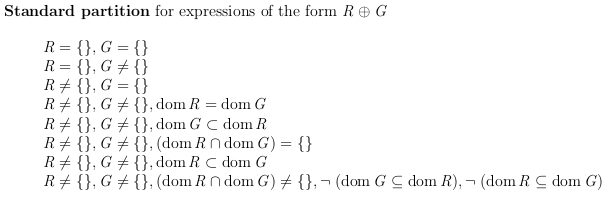
\includegraphics[scale=0.65]{particionoplus.png}
    \captionof{figure}{Partición estándar para expresiones de la forma $R \oplus G$ detallada en el manual de usuario de \textsc{Fastest}}
\end{center}

Entonces analicemos lo siguiente: 

\begin{itemize}
    \item como $G$ en nuestro caso resulta un conjunto con único elemento (la tupla $(course?, enrolledStudents(course?) \cup \{student?\})$, sabemos que no van a existir casos donde se pueda cumplir que $G = \{\}$.
    \item como $R = enrolledStudents$ y $course? \in \dom enrolledStudents$ sabemos que no van a existir casos donde $R = \{\}$.
    \item por los dos items anteriores sabemos que $(\dom R \cap \dom G) \neq \{\}$ pues ambas relaciones contienen en su dominio a $course?$. Entonces no podrá haber casos que se generen de tal manera.
    \item haciendo un análisis similar, como $\dom G$ es exactamente igual al conjunto con un único elemento $\{course?\}$ no puede ser verdad la contención estricta del dominio de $R$ en el dominio de $G$ por lo cual también descartamos el poder generar casos de prueba así.
    \item por último, siguiendo la misma lógica, no puede suceder que $\lnot(\dom G \subseteq \dom R)$ puesto que $\dom G = \{course?\}$ y sabemos que $course? \in \dom R$. Así que no existirán casos de prueba que cumplan con esta sentencia.
\end{itemize}

Por lo tanto, los únicos casos que sobreviven a la generación de casos de prueba son el cuarto y quinto de los mostrados en la imagen y esos son los que podremos ver luego.

\subsubsection*{Hojas de \texttt{EnrollStudent\_DNF\_2}}

Similar al caso anterior, podemos entender la partición de \verb|EnrolledStudent_DNF_2| como la partición generada por las precondiciones del siguiente esquema de Z:

\begin{schema}{EnrollStudentNewCourseOk}
    \Delta CourseManagementSystem \\
    student?: STUDENT \\
    course?: COURSE
    \where
    course? \in \dom(assignedProfessors) \\
    course? \nin \dom(enrolledStudents) \\
    enrolledStudents' = enrolledStudents \cup \{course? \mapsto \{student?\}\} \\
    assignedProfessors' = assignedProfessors
\end{schema}

Al aplicar el comando

\begin{verbatim}
    addtactic EnrollStudent_DNF_2 SP \cup 
        enrolledStudents \cup \{course? \mapsto \{student?\}\}
\end{verbatim}

se generarán 8 hijos desde el nodo \verb|EnrolledStudent_DNF_2| cada uno representando los 8 casos de la figura a continuación (tomando $S = enrolledStudents, T = \{course? \mapsto \{student?\}\}$).

\begin{center}
    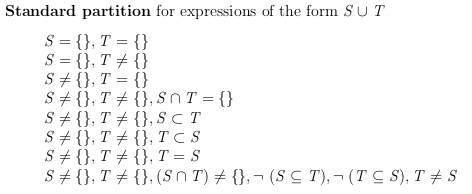
\includegraphics[scale=0.7]{particioncup.png}
    \captionof{figure}{Partición estándar para expresiones de la forma $S \cup T$ detallada en el manual de usuario de \textsc{Fastest}}
\end{center}

Entonces, otra vez analicemos:

\begin{itemize}
    \item como en nuestro caso $T = \{course? \mapsto \{student?\}\}$, entonces sabemos no se van a poder generar casos donde $T = \{\}$.
    \item como en nuestro caso $S = enrolledStudents$ y a su vez sabemos que $course? \notin \dom enrolledStudents$, sabemos que no puede existir ninguna tupla en $S$ con $course?$ como su primera componente. Como $T$ solo tiene el elemento que dimos en el ítem anterior, sabemos que no se podrán generar casos de prueba tales que $T = S$, ni tales que $S \cap T \neq \{\}$ (y, como consecuencia, ni tales que suceda alguna contención hacia algún lado con $S$ y $T$).
\end{itemize}

Por lo tanto, los únicos casos que sobreviven a la generación de casos de prueba son el segundo y el cuarto de los que se observan en la figura, y esos son los que veremos.

Con esto queda clara la razón por la cual \textsc{Fastest} no es capaz de generar casos de prueba para varias de las hojas del árbol que primero presentamos y por la cual obtenemos el segundo árbol que presentamos luego de aplicar \verb|genalltca|.

\subsection*{Esquemas Z de los casos de prueba generados}

Como último paso de este trabajo, se presentan los esquemas de casos de prueba abstractos generados por \textsc{Fastest}.

\begin{schema}{EnrollStudent\_ SP\_ 4\_ TCASE}\\
 EnrollStudent\_ SP\_ 4 
\where
 assignedProfessors = \{ ( cOURSE1 \mapsto \{ pROFESSOR2 \} ) \} \\
 course? = cOURSE1 \\
 enrolledStudents = \{ ( cOURSE1 \mapsto \emptyset ) \} \\
 student? = sTUDENT3
\end{schema}


\begin{schema}{EnrollStudent\_ SP\_ 5\_ TCASE}\\
 EnrollStudent\_ SP\_ 5 
\where
 assignedProfessors = \{ ( cOURSE1 \mapsto \{ pROFESSOR3 \} ) \} \\
 course? = cOURSE1 \\
 enrolledStudents = \{ ( cOURSE1 \mapsto \emptyset ) , ( cOURSE2 \mapsto \{ sTUDENT1 , sTUDENT2 \} ) \} \\
 student? = sTUDENT5
\end{schema}


\begin{schema}{EnrollStudent\_ SP\_ 10\_ TCASE}\\
 EnrollStudent\_ SP\_ 10 
\where
 assignedProfessors = \{ ( cOURSE1 \mapsto \{ pROFESSOR2 \} ) \} \\
 course? = cOURSE1 \\
 enrolledStudents =~\emptyset \\
 student? = sTUDENT3
\end{schema}


\begin{schema}{EnrollStudent\_ SP\_ 12\_ TCASE}\\
 EnrollStudent\_ SP\_ 12 
\where
 assignedProfessors = \{ ( cOURSE1 \mapsto \{ pROFESSOR2 \} ) \} \\
 course? = cOURSE1 \\
 enrolledStudents = \{ ( cOURSE2 \mapsto \{ sTUDENT1 \} ) \} \\
 student? = sTUDENT3
\end{schema}


\begin{schema}{EnrollStudent\_ SP\_ 17\_ TCASE}\\
 EnrollStudent\_ SP\_ 17 
\where
 assignedProfessors =~\emptyset \\
 course? = cOURSE2 \\
 enrolledStudents =~\emptyset \\
 student? = sTUDENT1
\end{schema}


\begin{schema}{EnrollStudent\_ SP\_ 18\_ TCASE}\\
 EnrollStudent\_ SP\_ 18 
\where
 assignedProfessors = \{ ( cOURSE2 \mapsto \{ pROFESSOR1 \} ) \} \\
 course? = cOURSE1 \\
 enrolledStudents =~\emptyset \\
 student? = sTUDENT2
\end{schema}


\begin{schema}{EnrollStudent\_ SP\_ 19\_ TCASE}\\
 EnrollStudent\_ SP\_ 19 
\where
 assignedProfessors = \{ ( cOURSE1 \mapsto \{ pROFESSOR1 , pROFESSOR2 \} ) \} \\
 course? = cOURSE1 \\
 enrolledStudents = \{ ( cOURSE1 \mapsto \{ sTUDENT2 \} ) \} \\
 student? = sTUDENT2
\end{schema}


\begin{schema}{EnrollStudent\_ SP\_ 20\_ TCASE}\\
 EnrollStudent\_ SP\_ 20 
\where
 assignedProfessors = \{ ( cOURSE1 \mapsto \{ pROFESSOR2 \} ) \} \\
 course? = cOURSE1 \\
 enrolledStudents = \{ ( cOURSE1 \mapsto \{ sTUDENT1 , sTUDENT2 \} ) \} \\
 student? = sTUDENT1
\end{schema}

\end{document}

